\subsection{Early Warning Indicators chap3}

 




\subsubsection{Definition}
\begin{itemize}
\item Early warning indicators (EWls) are analogous to warning lights on a car dashboard.
\item EWIs are changes in key metrics (qualitative or quantitative) that could signal a pending liquidity problem and they can vary in severity and priority.
\end{itemize}



\subsubsection{EWI \& Liquidity risk management process (LRM)}
\begin{itemize}
\item LRM framework begins by identifying liquidity and funding risks that are inherent in the business activities.
\item LRM framework should be end-to-end and ensure that the bank will "sufficiently capture the banking organization's exposures, activities, and risks."
\item Ensure that EWls are updated and aligned with other core aspects of the LRM framework.
\item Ensure the quality and timeliness of the data that feeds into the EWIs.
\end{itemize}



\subsubsection{Framework Components: M.E.R.I.T}
\begin{itemize}
\item Measures
    \begin{itemize}
    \item Measures should be leading and sharp.
        \begin{itemize}
        \item Leading(forward looking): provide information and signal potential stress prior to the occurrence of an actual event.
        \item Sharp(sufficiently granular): signals do not go unnoticed within the mass of data.
        \end{itemize}
    \item Measures should contain both external and internal measures.
        \begin{itemize}
        \item Internal measures: customize bank's B/S and activities.
        \item External measures: signal systemic changes in the economy or market.
        \end{itemize}
    \end{itemize}
    
\item Escalation
    \begin{itemize}
    \item An effective escalation policy should ensure that limit breaches are escalated to the appropriate level of management with the authority to undertake corrective actions.
        \begin{itemize}
        \item Modest response: increase liquid asset buffer
        \item Large cash outflow from EWI: asset-liability committee (ALCO)
        \item Extreme cases: contingency funding plan (CFP)
        \end{itemize}
    \end{itemize}
    
\item Reporting
    \begin{itemize}
    \item EWI report needs to be timely in order to provide management with sufficient lead time to make adjustment in response to potential crisis events. It is common practice to have the EWI dashboard reported on a daily basis.
    \end{itemize}
    
\item Integrated systems
    \begin{itemize}
    \item Metrics and reporting are feasible and meaningful only when they are backed by the bank's ability to calculate the selected metrics and report them consistently.
    \end{itemize}
    
\item Thresholds
    \begin{itemize}
    \item Firms use a stoplight system in represent and communicate performance against the thresholds of their EWls.
        \begin{itemize}
        \item Green indicator: the measure is within normal bounds.
        \item Amber indicator: the measure should be investigated further.
        \item Red indicator: significant concern and may need an immediate response.
        \end{itemize}
    \item The threshold boundaries for which an EWI moves from green to amber should not be too wide or too narrow.
        \begin{itemize}
        \item Use back-testing to determine if recalibration is needed.
        \end{itemize}
    \end{itemize}
    
\end{itemize}



\subsubsection{Guidelines from OCC}
\begin{itemize}
\item EWI may include but not limited to the items listed below:
    \begin{itemize}
    \item A reluctance of traditional fund providers to continue funding at historic levels.
    \item Pending regulatory action(both formal and informal) or CAMELS component or composite rating downgrade(s).
        \begin{itemize}
        \item CAMELS: capital, asset quality, management, earnings, liquidity, and sensitivity.
        \end{itemize}
    \item Widening of spreads on debts, credit default swaps, and stock price declines.
    \item Difficulty in accessing long-term debt markets.
    \item Reluctance of trust managers, money managers, public entities, and credit-sensitive funds providers to place funds.
    \item Rising funding costs in an otherwise-stable market.
    \item Counterparty resistance to off-balance-sheet products or increased margin requirements.
    \item The elimination of committed credit lines by counterparties.
    \end{itemize}
\end{itemize}



\subsubsection{Guidelines from BCBS}
\begin{itemize}
\item EWI may include but not limited to the items listed below:
    \begin{itemize}
    \item Rapid asset growth, especially when funded with potentially volatile liabilities.
    \item Growing concentrations in assets or liabilities.
    \item Increases in currency mismatches.
    \item Decrease of weighted average maturity of liabilities.
    \item Repeated incidents of positions approaching or breaching internal or regulatory limits.
    \item Negative trends or heightened risk associated with a particular product line.
    \item Negative publicity
    \item Credit rating downgrade
    \item Stock price declines
    \item Rising debt costs
    \item Widening debt/credit-default-swap spreads
    \item Rising wholesale/retail funding costs
    \item Counterparties requesting additional collateral or resisting entering into new transactions
    \item Drop in credit lines
    \item Increasing retail deposit outflows
    \item Increasing redemptions of CDs before maturity
    \item Difficulty accessing longer-term funding
    \item Difficulty placing short-term liabilities
    \end{itemize}
\item Intraday liquidity monitoring indicators include:
    \begin{itemize}
    \item Daily maximum liquidity requirement
    \item Available intraday liquidity
    \item Total payments
    \item Time-specific and other critical obligations
    \item Value of customer payments made on behalf of financial institutions customers
    \item Intraday credit lines extended to financial institution customers
    \item Timing of intraday payments
    \item Intraday throughput
    \end{itemize}
\end{itemize}



\subsubsection{Guidelines from Federal Reserve}
\begin{itemize}
\item EWI may include but not limited to the items listed below:
    \begin{itemize}
    \item Negative publicity concerning an asset class owned by the institution.
    \item Increased potential for deterioration in the institution's financial condition.
    \item Widening debt or credit default swap spreads.
    \item Increased concerns over the funding of off-balance-sheet items
    \end{itemize}
    
\end{itemize}


\subsection{Intraday Liquidity Risk Management Ch6}

\subsubsection{Basics of intradav liauiditv}
\begin{itemize}
\item A bank treasurer manages intraday liquidity risk and enumerates the sources and uses of intraday funds for a typical large bank.
    \begin{itemize}
    \item Target: Ensure the bank remains within the limits of its daylight credit resources and ends the day with the appropriate target balances in its accounts.
    \item Challenges: factors of intraday funds management target
        \begin{itemize}
        \item Variability of cash flow patterns
        \item Impact of market forces
        \item Lack of real-time data
        \end{itemize}
    
    \end{itemize}
    
\end{itemize}



\subsubsection{Uses of intraday liquidity fund}
\begin{itemize}
\item Outgoing Wire Transfers (largest use of intraday liquidity)

\begin{table}[htbp]
    \centering
    \begin{tabular}{@{}ll@{}}
        \toprule
        Description & \checkmark Payments on LVPS such as Fedwire and CHIPS \\
        \midrule
        Impacted by client activity & \makecell{\checkmark Yes \\ \checkmark Clients provide bank instructions} \\
        \midrule
        Impacted by bank activity & \makecell{\checkmark Yes \\ \checkmark Bank treasury and lines of business have payment needs} \\
        \midrule
        Ability to forecast & \makecell{\checkmark Bank activity can usually be forecasted with 1 to 2 days' notice \\ \checkmark client payment activity is more difficult to predict} \\
        \bottomrule
    \end{tabular}
\end{table}
\item Settlements at PCS systems



\begin{table}[H]
    \centering
    \begin{tabular}{@{}ll@{}}
        \toprule
        Description & \checkmark Net cash settlements at payments systems, clearing houses \\
        \midrule
        Impacted by Client Activity & \makecell{\checkmark Not directly initiated by clients, but includes client activity} \\
        \midrule
        Impacted by Bank Activity & \makecell{\checkmark Yes \\ \checkmark Position monitored by operations groups} \\
        \midrule
        Ability to forecast & \makecell{\checkmark Can be forecast for securities that have multi-day settlements (e.g., T +3) \\ \checkmark More difficult same day settlement activity} \\
        \bottomrule
    \end{tabular}
\end{table}
\item Funding Nostro Accounts

\begin{table}[htbp]
    \centering
    \begin{tabular}{@{}ll@{}}
        \toprule
        Description & \checkmark Cash transfer to a correspondent bank for services provided \\
        \midrule
        Impacted by Client Activity & \makecell{\checkmark Not directly initiated by clients, but includes client activity} \\
        \midrule
        Impacted by Bank Activity & \makecell{\checkmark Yes \\ \checkmark Position monitored by operations groups} \\
        \midrule
        Ability to forecast & \makecell{\checkmark Securities settlements are generally predictable \\ \checkmark Client payment activity flowing through correspondents is less predictable} \\
        \bottomrule
    \end{tabular}
\end{table}
\item Collateral Pledging

\begin{table}[htbp]
    \centering
    \begin{tabular}{@{}ll@{}}
        \toprule
        Description & \checkmark Obtaining and earmarking of collateral required by an outside beneficiary \\
        \midrule
        Impacted by Client Activity & \makecell{\checkmark Yes \\ \checkmark some clients require collateral to cover bank trading liabilities or deposits} \\
        \midrule
        Impacted by Bank Activity & \makecell{\checkmark Yes \\ \checkmark banks are required to post collateral for margin at FMUs other trading counterparties} \\
        \midrule
        Ability to forecast & \checkmark Dependent on trading volumes and asset price changes, generally known one day in advance \\
        \bottomrule
    \end{tabular}
\end{table}
\item Asset Purchases/Funding

\begin{table}[htbp]
    \centering
    \begin{tabular}{@{}ll@{}}
        \toprule
        Description & \checkmark Exchange of bank cash for another asset such as a client loan \\
        \midrule
        Impacted by Client Activity & \makecell{\checkmark Yes \\ \checkmark Clients can draw down on lines of credit or letters of credit} \\
        \midrule
        Impacted by Bank Activity & \makecell{\checkmark Yes \\ \checkmark Assets may be securities for the bank’s investment portfolio or fixed assets} \\
        \midrule
        Ability to forecast & \makecell{\checkmark Bank fixed asset activity should be known in advance \\ \checkmark Securities purchases may be same day settlement \\ \checkmark Client loans are more difficult to predict} \\
        \bottomrule
    \end{tabular}
\end{table}
\end{itemize}



\subsubsection{Sources of intraday liquidity fund}
\begin{itemize}
\item Cash Balances

\begin{table}[htbp]
    \centering
    \begin{tabular}{@{}ll@{}}
        \toprule
        Description & \checkmark Deposits at central bank and correspondent bank nostro accounts \\
        \midrule
        Impacted by Client Activity & \makecell{\checkmark No \\ \checkmark clients do not directly impact closing/start of day cash balances} \\
        \midrule
        Impacted by Bank Activity & \makecell{\checkmark Yes \\ \checkmark Bank Treasury determines level of closing/start of day cash balances} \\
        \midrule
        Ability to forecast & \makecell{\checkmark Bank activity can usually be forecasted with 1 to 2 days' notice \\ \checkmark Client payment activity is more difficult to predict} \\
        \bottomrule
    \end{tabular}
\end{table}
\item Incoming Funds Flow

\begin{table}[htbp]
    \centering
    \begin{tabular}{@{}ll@{}}
        \toprule
        Description & \checkmark Incoming cash payments and cash credits from FMU \\
        \midrule
        Impacted by Client Activity & \makecell{\checkmark Yes \\ \checkmark Incoming client payments are credited to the bank's accounts at the central bank and correspondents} \\
        \midrule
        Impacted by Bank Activity & \makecell{\checkmark Yes \\ \checkmark Activities conducted for the bank's business can impact cash balances} \\
        \midrule
        Ability to forecast & \makecell{\checkmark Bank activity can usually be forecasted with 1 to 2 days' notice \\ \checkmark Client payment activity is more difficult to predict. \\ \checkmark FMU credit can be forecast for securities that have multi - day settlements (e.g., T + 3) and more difficult same day settlement activity} \\
        \bottomrule
    \end{tabular}
\end{table}
\item lntraday credit

\begin{table}[htbp]
    \centering
    \begin{tabular}{@{}ll@{}}
        \toprule
        Description & \makecell{\checkmark Credit line or overdraft permitted during business hours and covered by close of business. \\ \checkmark Lines are often uncommitted and provided without interest charges.} \\
        \midrule
        Impacted by Client Activity & \checkmark No, client activity does not directly impact the amount of intraday credit extended to a bank \\
        \midrule
        Impacted by Bank Activity & \makecell{\checkmark Yes \\ \checkmark Counterparties will often adjust intraday credit extensions to reflect business activity from other areas of the bank(e.g., OTC trading)} \\
        \midrule
        Ability to forecast & \makecell{\checkmark Some intraday credit facilities are disclosed and well known to a bank. \\ \checkmark Others are not disclosed but can often be inferred from historical data} \\
        \bottomrule
    \end{tabular}
\end{table}
\item Liquid Assets

\begin{table}[htbp]
    \centering
    \begin{tabular}{@{}ll@{}}
        \toprule
        Description & \makecell{\checkmark Cash, money market deposits, and short-term government debt (e.g., Bills) which can be quickly converted to cash} \\
        \midrule
        Impacted by Client Activity & \makecell{\checkmark Yes \\ \checkmark Client may be sources of liquidity in converting liquid assets to cash (e.g., repo transaction)} \\
        \midrule
        Impacted by Bank Activity & \makecell{\checkmark Yes \\ \checkmark Bank trading and investment portfolio activity can impact the amount of liquid assets available.} \\
        \midrule
        Ability to forecast & \checkmark Liquid assets held in the investment portfolio and in other money market investments tend to have \textcolor{blue}{low volatility and as a result are predictable} \\
        \bottomrule
    \end{tabular}
\end{table}
\item Overnight Borrowings

\begin{table}[htbp]
    \centering
    \begin{tabular}{@{}ll@{}}
        \toprule
        Description & \makecell{\checkmark Fed Funds \\ \checkmark Eurodollar borrowing \\ \checkmark Overnight deposits} \\
        \midrule
        Impacted by Client Activity & \makecell{\checkmark Yes \\ \checkmark Clients may be direct sources of liquidity for overnight borrowing (e.g.,. overnight deposit)} \\
        \midrule
        Impacted by Bank Activity & \makecell{\checkmark No \\ \checkmark Other bank lines of business do not regularly supply overnight funding} \\
        \midrule
        Ability to forecast & \checkmark Client supply of overnight borrowing tends to be fairly predictable, but with \textcolor{blue}{moderate volatility} \\
        \bottomrule
    \end{tabular}
\end{table}
\item Other Term Funding

\begin{table}[htbp]
    \centering
    \begin{tabular}{@{}ll@{}}
        \toprule
        Description & \makecell{\checkmark Other term deposits \\ \checkmark Repos from FHLB \\ \checkmark Money market funds, etc.} \\
        \midrule
        Impacted by Client Activity & \makecell{\checkmark Yes \\ \checkmark Clients may be direct sources of liquidity for term funding} \\
        \midrule
        Impacted by Bank Activity & \makecell{\checkmark No \\ \checkmark Other bank lines of business do not regularly supply term funding} \\
        \midrule
        Ability to forecast & \checkmark Client supply of term funding tends to be predictable, but with \textcolor{blue}{low volatility} \\
        \bottomrule
    \end{tabular}
\end{table}
\end{itemize}



\subsubsection{Governance of lntraday LRM}
\begin{itemize}
\item Active risk management
    \begin{itemize}
    \item Classify settlement and systemic risks as components of risk taxonomy, and critically, incorporate these risks into the firm's risk appetite framework.
    \end{itemize}
    
\item Integration with risk governance: Oversight of intraday liquidity risk management is integrated into the bank's overall risk oversight structure. Three lines of defense model:
    \begin{itemize}
    \item Treasury: manages the intraday funding positions of risk management programs related to funding activities.
    \item Corporate Risk Management: oversees funding-related policy and procedures.
    \item Internal Audit: independently assesses the bank's adherence to intraday risk policies and procedures.
    \end{itemize}
    
\item Risk assessment
    \begin{itemize}
    \item Through risk self-assessments, settlement risks related to existing and potential new products and operational processes are identified, measured, and evaluated.
    \end{itemize}
    
\item Risk measurement and monitoring
    \begin{itemize}
    \item The amount of intraday credit the institution is extending to clients.
    \item The amount of intraday credit the institution utilizes.
    \end{itemize}
    
\end{itemize}



\subsubsection{Measures for understanding intraday flows}
\begin{itemize}
\item Total payments
    \begin{itemize}
    \item A bank and its intraday risk management should maintain statistic concerning the amount of payments it makes on all electronic payments systems in which it participants.
    \item For example:
        \begin{itemize}
        \item Total payments sent and received for non-financial institution or financial institution clients/ bank activity.
        \item Net position in the settlement account at any time of day in aggregate.
        \end{itemize}
        
    \end{itemize}
    
\item Other cash transactions
    \begin{itemize}
    \item A bank should also track its intraday and end-of-day settlement positions at all financial market utilities in which it participates, such as collateral position in SSN.
    \end{itemize}
    
\item Settlement positions
    \begin{itemize}
    \item If complete data to reconstruct account positions at any time of day is not available, at a minimum a bank should maintain data on its settlement positions with all its FMUs.
    \end{itemize}
    
\item Time sensitive obligations
    \begin{itemize}
    \item For those transactions require completion at a specific time during the day, such as return of borrowing, margin payments. Failure to settle may result in a financial penalty.
    \end{itemize}
    
\item Total intraday credit lines to clients and counterparties
    \begin{itemize}
    \item Bank should have data regarding average and peak usage, and the ability to model activity at the client and portfolio levels.
    \end{itemize}
    
\item Total bank intraday credit lines available and usage
    \begin{itemize}
    \item The amount of intraday credit that a bank relies on in business-as-usual conditions and the maximum amount of intraday borrowing it can draw down.
    \item Captures the amount of committed and uncommitted intraday credit (and usage thereof) the bank has at its disposal, ideally across all its cash and settlement accounts.
    \end{itemize}
    
\end{itemize}



\subsubsection{Measures for quantifying and monitoring risk levels}
\begin{itemize}
\item Daily maximum intraday liquidity usage
    \begin{itemize}
    \item Formula: $\dfrac{\text{the day's largest negative balance}}{\text{the size of the committed or uncommitted credit line}}$
        \begin{itemize}
        \item This calculation does not need real-time monitoring of an account to capture all of the negative positions.
        \end{itemize}
    \item Typically, the peak and average of this metric is tracked over a period of time (e.g. monthly).

    \end{itemize}
    
\item Intraday credit relative to tier 1 capital
    \begin{itemize}
    \item Formula: $\dfrac{\text{Intraday credit}}{\text {Tier 1 capital}}$
        \begin{itemize}
        \item The measure should be tracked for total intraday credit and unsecured intraday credit, available and used.
        \item Represents the intraday settlement risk.
        \end{itemize}
    \item Available unsecured intraday credit relative to an institution's tier 1 capital is a rough measure of the inadvertent systemic risk that the institution poses to the financial system.

    \end{itemize}
\item Client intraday credit usage
    \begin{itemize}
    \item Formula: $\dfrac{\text{Client's peak daily intraday overdraft}}{\text {established ( committed or uncommitted) credit line}}$
    \item Provides useful insights for understanding how client activity impacts the bank's ability to manage its own
    intraday liquidity
    \end{itemize}
    
\item Payment throughput
    \begin{itemize}
    \item These measures track the percentage of outgoing payment activity relative to time of day.
    \item Help the bank identify and monitor its peak periods over time and the correlation of this activity with its intraday liquidity on hand and intraday credit usage.
    \end{itemize}
    
\end{itemize}

\subsection{liquidity Stress Testing and Reporting Ch9}


\subsubsection{Four categories of funding liquidity}
\begin{itemize}
\item Operational liquidity: The cash that is needed to fund the business daily.
    \begin{itemize}
    \item May be quite volatile
    \item May need cushion for unpredictability of daily settlement
    \end{itemize}
\item Restricted liquidity: Liquid assets only for specifically defined purpose, such as collateralization.
    \begin{itemize}
    \item Unavailable to meet general financial obligations under a liquidity stress test.
    \end{itemize}
\item Strategic liquidity: The cash that is held by the institution to meet future business needs, outside the course of normal operations.
    \begin{itemize}
    \item Fixed asset purchases or M\&A
    \end{itemize}
\item Contingent liquidity: Liquid asset buffer composed of high quality and liquid financial assets.
    \begin{itemize}
    \item Meet general financial obligations under a stress scenario.
    \end{itemize}
\end{itemize}
\begin{center}
    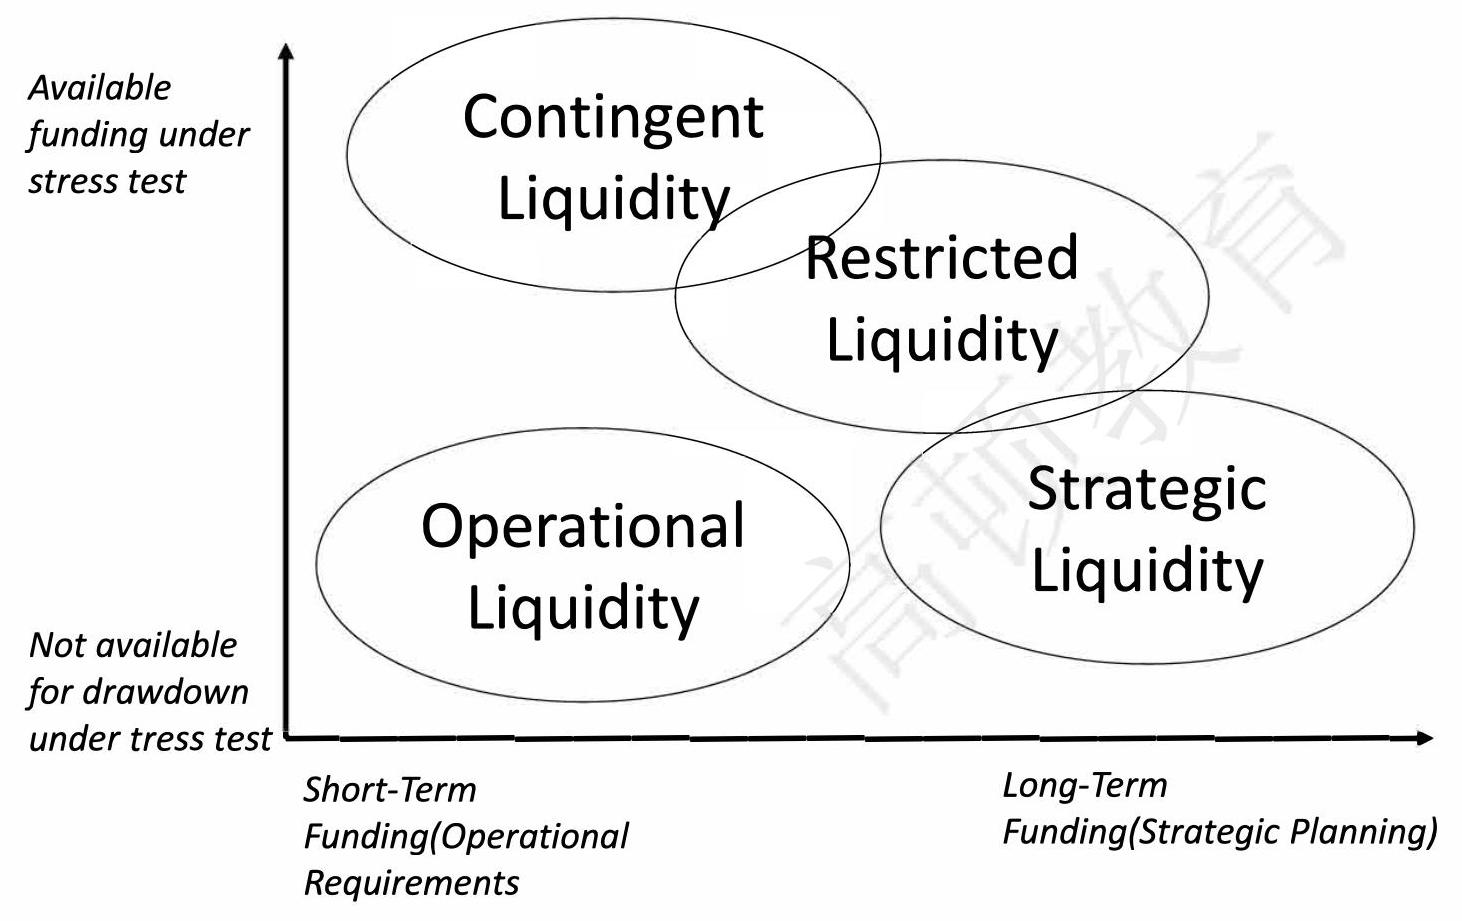
\includegraphics[width=0.9\textwidth]{images/funding li.jpg}
    \end{center}


\subsubsection{Estimating stressed liquidity asset buffer}
\begin{itemize}
\item Stressed liquidity asset buffer: indicates the adequacy of the current liquid asset buffer given stress scenario assumptions.
\item Calculation formular:
    \begin{itemize}
    \item stressed liquidity asset buffer = normal liquidity asset buffer - stressed cash outflow + stressed cash inflow
        \begin{itemize}
        \item Normal liquidity asset buffer: the amount of contingent liquidity currently held.
        \item Stressed outflow: require early settlement of liabilities or the inability to rollover debt.
        \item Stressed inflows: such as drawdowns on liquidity facilities available to the institution.
        \end{itemize}
        
    \end{itemize}
\item Example
    \begin{itemize}
    \item Bank ABC has 1 million dollars in highly liquid asset. In its stressed scenario assumption, the retail customer will withdraw \$200,000 deposit and the debt cannot roll over is \$600,000. The bank can use the remaining \$500,000 of its available liquidity facility. What is the estimate stressed liquid asset buffer?
    \item Answer:
        \begin{itemize}
        \item 1,000,000-(200,000+600,000)+500,000=700,000 dollars
        \end{itemize}
        
        
    \end{itemize}
    
    
\end{itemize}



\subsubsection{Design of the model}
\begin{itemize}
\item Organizational scope
\item Scenario development
\item Development of assumptions
\item Outputs of the model
\item Governance and controls
\item Integrations with other risk models
\end{itemize}



\subsubsection{Organizational scope}
\begin{itemize}
\item Liquidity transfer restrictions
    \begin{itemize}
    \item Liquidity may be trapped in certain legal entities and cannot be transferred freely throughout the organization
    \end{itemize}
\item Currency
    \begin{itemize}
    \item Perform liquidity stress test in the currency of the entity being tested, and take liquidity impact of currency conversion requirements for consideration
    \end{itemize}
\item Regulatory jurisdiction
    \begin{itemize}
    \item Perform separate stress tests for the foreign entities
    \end{itemize}
    
\end{itemize}



\subsubsection{Scenario development}
\begin{itemize}
\item Historical scenarios
    \begin{itemize}
    \item Historical scenarios are based on actual liquidity failures and attempt to translate those events to the financial institution performing the stress test.
    \item Disadvantage:
        \begin{itemize}
        \item The existence of few examples with limited data
        \item The past is not always indicative of the future
        \end{itemize}
        
    \item Forward-looking view in which the financial institution experiences severe liquidity stress:
        \begin{itemize}
        \item Distinguish between systemic and idiosyncratic risk
        \item Distinguish between levels of severity.
        \item Clearly define the scenarios.
        \end{itemize}
        
    \item Reverse liquidity stress tests: supplement to hypothetical scenanos.
    \end{itemize}

\end{itemize}



\subsubsection{Development of Assumptions}
\begin{itemize}
\item Develops liquidity stress testing assumptions the institution should do the following:
    \begin{itemize}
    \item Qualitatively assess the expected liquidity behavior for each type of cash flow to determine where there is significant liquidity risk.
    \item Determine the appropriate level of segmentation for each type of risk based on an assessment of behavioral differences, bearing in mind any limitations in ongoing data availability.
    \item Qualitatively assess and order by rank varying levels of liquidity risk for each segmentation factor, potentially utilizing a scoring system.
    \item Develop quantitative modeling assumptions based on any historical data available, such as experiences during the financial crisis, or available from other sources such as peer benchmarking.
    \item Develop matrices of relative modeling assumptions based on scored risk levels and baseline historical data.
    \item Adjust assumption matrices as appropriate for each stress scenario, for example, reflecting differences in relative overall severity or assumptions concerning idiosyncratic or systemic risk.
    \end{itemize}
    
\item The following assumptions can have an outsized impact on the results of the stress test, and should be considered carefully in developing the model:
    \begin{itemize}
    \item Investment portfolio haircuts
    \item Deposit outflows
    \item Unsecured wholesale funding
    \item Collateral requirements
    \item Other contingent liabilities
    \item Business dial back
    \end{itemize}
    
\end{itemize}



\subsubsection{Outputs of the model}
\begin{itemize}
\item Stress testing assumptions
    \begin{itemize}
    \item Overall stress level by the scenarios
    \item Indication of whether the scenario is systemic, idiosyncratic, or both
    \item Contribution of economic, market, and firm-specific events
    \item Cash flows resulting from the scenario
    \end{itemize}
\item Liquidity position metrics
    \begin{itemize}
    \item Main objective is to determine how much liquidity is available compared to the net cash outflows.
    \end{itemize}
\item Prospective liquidity position metrics
    \begin{itemize}
    \item Highlight any times during the stress horizon where survival would require significant transactions such as capital infusion and debt issuances.
    \end{itemize}
\item Capital and performance metrics
    \begin{itemize}
    \item Captures the impact of any capital actions required to support liquidity during the stress period.
    \end{itemize}
\end{itemize}



\subsubsection{Governance and controls}
\begin{itemize}
\item Asset-liability committee(ALCO)
    \begin{itemize}
    \item The ALCO is in charge of the liquidity stress testing framew ork.
    \item Ensuring the establishment, review, and approval of a liquidity stress testing policy.
    \item Suggesting and approving liquidity risk scenarios.
    \item Setting liquidity risk policy limits dependent on stress test outcomes.
    \end{itemize}
\item Treasury unit ( the first line of defense)
    \begin{itemize}
    \item Maintenance of liquidity stress testing procedures.
    \item Recommending stress test scenarios.
    \item Analyzing liquidity characteristics of the assets and liabilities.
    \item Recommend assumptions used in stress testing to ALCO.
    \item Reports results of stress testing.
    \end{itemize}
\item Risk management department ( the second line of defense)
    \begin{itemize}
    \item Administering the liquidity risk stress testing policy
    \item Reviewing and providing effective challenge of the scenario design and assumptions
    \item Ensuring the institution's approach to liquidity stress testing is in line with acceptable industry practices and regulatory rules and guidance
    \item Reviewing and approving the liquidity stress test-based limits
    \item Monitoring of liquidity stress test-based limits
    \item Ensuring the institution's ALCO, executive management, and board are kept well-informed of the bank's liquidity risk profile as indicated by the stress testing results
    \end{itemize}
\item Internal audit ( the third line of defense)
    \begin{itemize}
    \item Regular checks on the stress testing process, procedures, and controls as a confirmation.
    \end{itemize}
\item Model risk management
    \begin{itemize}
    \item A separate group that validates the stress testing model to ensure it is consistent with the firm's model risk management policy.
    \end{itemize}
\end{itemize}




\subsubsection{Integrations with other risk models}
\begin{itemize}
\item Liquidity stress testing and capital stress testing:
    \begin{itemize}
    \item Liquidity stress test incorporates any required capital infusions of subsidiary entities. Capital stress testing should consider liquidity stress evaluation.
    \end{itemize}
\item Liquidity stress testing and asset liability management:
    \begin{itemize}
    \item Liquidity stress test scenario framework, and liquidity risk EWIs should not neglect to include the possibility of an interest rate shock and the potential impact such an event would have on indeterminate liabilities.
    \end{itemize}
\item Liquidity stress testing and funds transfer pricing:
    \begin{itemize}
    \item Cost of carrying cash buffer required in liquidity stress testing will be priced through FTP framework.
    \end{itemize}
\end{itemize}



\subsubsection{Liquidity Stress test report}
\begin{itemize}
\item Definition: Stress test output results (report)
    \begin{itemize}
    \item Help senior management to understand the liquidity position of the bank, enabling them to take mitigating action if deemed necessary.
        \begin{itemize}
        \item Cash flow survival report
        \item Stressed cumulative cash flow forecast
        \item Line-by-line stress test result report
        \end{itemize}
        
    \end{itemize}
\end{itemize}



\subsubsection{Cash flow survival report}
\begin{itemize}
\item The primary stress test output:
    \begin{itemize}
    \item A report under business as usual (BAU) conditions and one after taking the mitigating actions (such as liquidating securities, and accessing contingency funding sources).
    \item Frequency: weekly for firm-specific/daily for market-wide.
    \end{itemize}
\end{itemize}
\begin{center}
    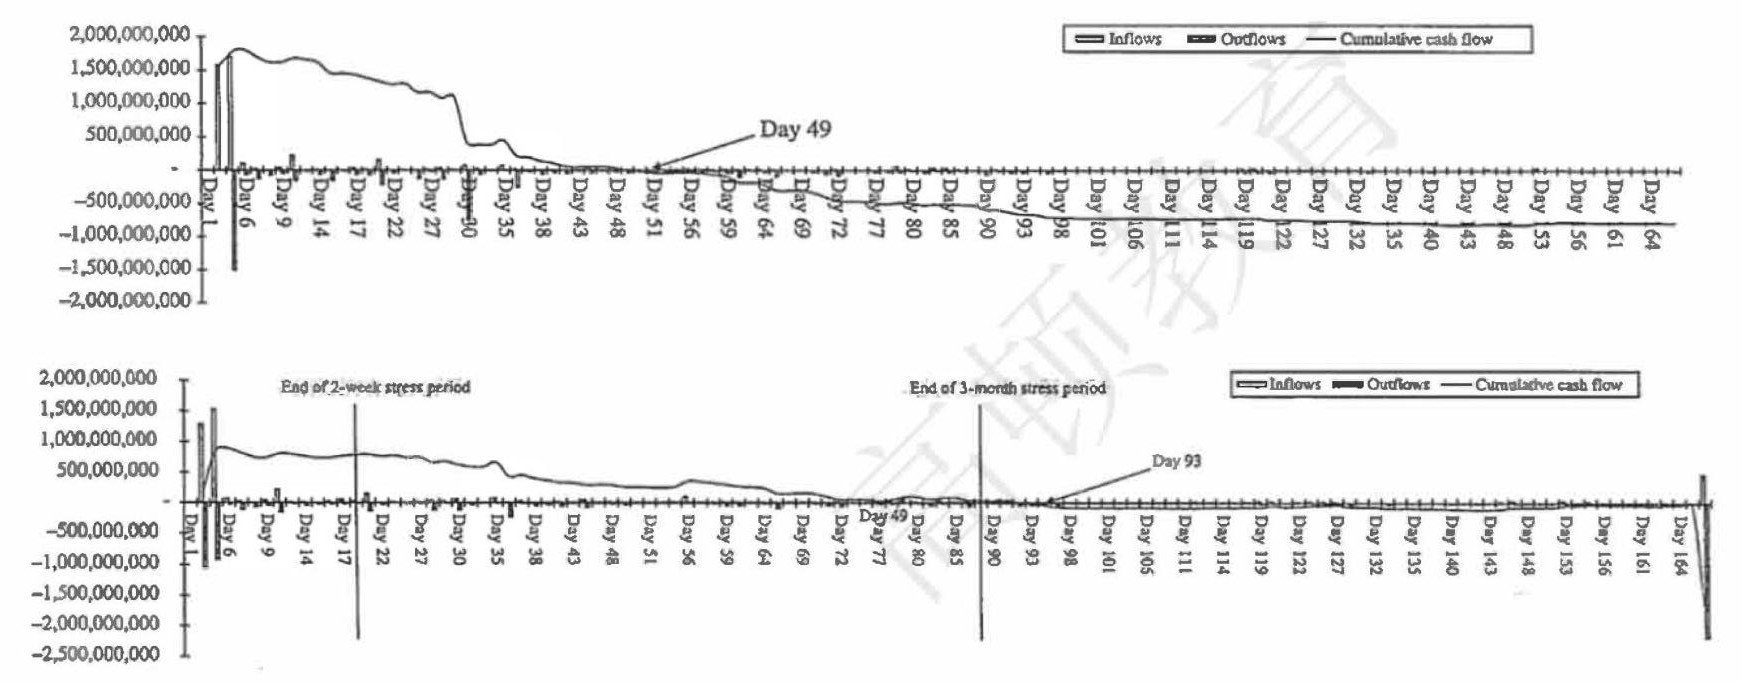
\includegraphics[width=0.9\textwidth]{images/survival report (2).jpg}
    \end{center}

    
\subsubsection{Stressed cumulative cash flow forecast}
\begin{itemize}
\item The second stress test output shows the stressed cumulative cash flow forecast taking into account the immediate sale repo of marketable securities.
\end{itemize}
\begin{minipage}[c]{0.45\textwidth}
    \centering
    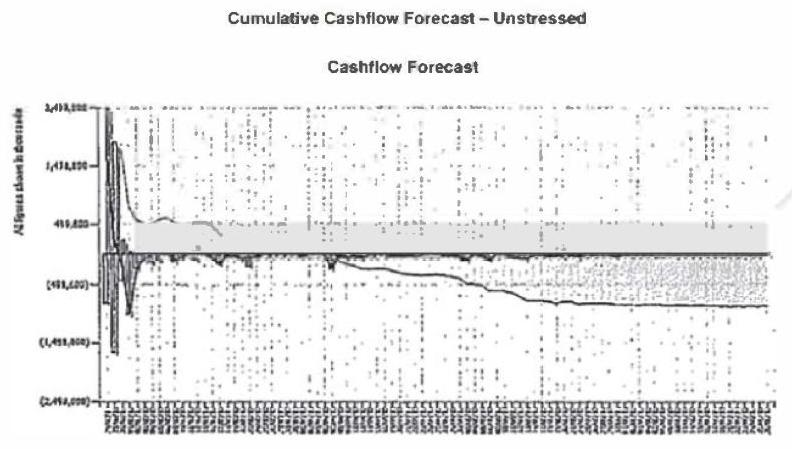
\includegraphics[width=\textwidth]{images/cashflow forecast1.jpg}
\end{minipage}
\hfill % 起到水平间距调整，让两图尽量分开
\begin{minipage}[c]{0.45\textwidth}
    \centering
    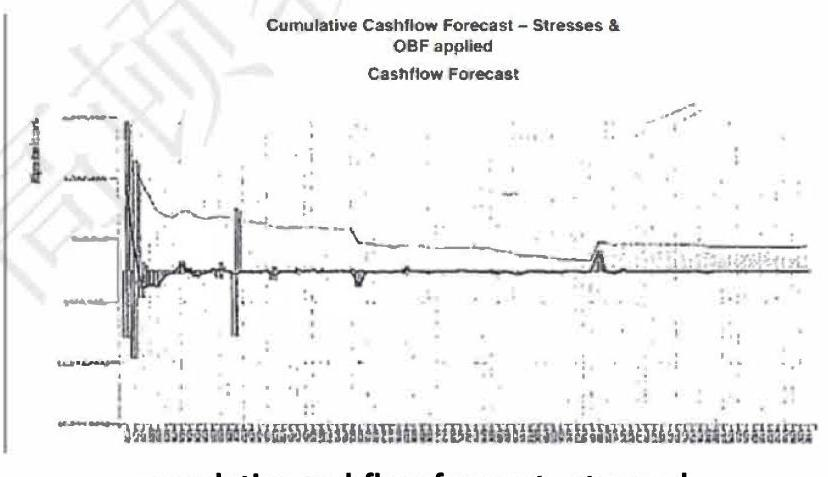
\includegraphics[width=\textwidth]{images/cashflow forecast2.jpg}
\end{minipage}
        

\subsubsection{Line-by-line stress test result report}
\begin{itemize}
\item Show the results of individual shocks on the liquidity ratio, and the probability of each result occurring and is a part of routine stress testing undertaken by Treasury or Risk Management.
    \begin{itemize}
    \item Individual shocks like:
        \begin{itemize}
        \item Reduction in liquid assets
        \item Decrease in liabilities
        \item FX mismatch
        \end{itemize}
    \item Frequency: quarterly or required by the regulator.
    \end{itemize}
\item Reduction in liquid assets


\begin{table}[ht]
    \centering
    \small
    \begin{tabular}{|c|m{1.5cm}|m{3cm}|m{1.5cm}|m{1.5cm}|m{1.5cm}|m{1.5cm}|}
    \hline
    \textbf{Reduction in Liquid Assets} & \textbf{Severity} & \textbf{Description} & \textbf{Sight – 8 Day} & \textbf{Sight – 1 Month} & \textbf{Probability} & \textbf{Impact} \\
    \hline
    \multirow{3}{*}{Change in repo criteria} 
      & Light & Rating category 1 notch downgrade & 8.46\% & 1.35\% & 50\% & 30 \\
      & Moderate & Rating category 2 notch downgrade & 2.34\% & 0.12\% & 20\% & 70 \\
      & Severe & Rating category 3 notch downgrade & -15.2\% & -18.2\% & 1\% & 90 \\
    \hline
    \multirow{3}{*}{Mark-to-market reduction in value of assets} 
      & Light &  & 8.46\% & 1.35\% & 60\% & 20 \\
      & Moderate &  & 2.34\% & 0.12\% & 40\% & 30 \\
      & Severe &  & -15.2\% & -18.2\% & 5\% & 70 \\
    \hline
    \multirow{3}{*}{Increased haircut on assets} 
      & Light &  & 8.46\% & 1.35\% & 70\% & 25 \\
      & Moderate &  & 2.34\% & 0.12\% & 30\% & 45 \\
      & Severe &  & -15.2\% & -18.2\% & 8\% & 80 \\
    \hline
    Unavailability of repo facilities 
      & Severe & Treat all marketable securities as illiquid (i.e., allocate to final legal maturity time buckets) & -15.2\% & -18.2\% & 5\% & 100 \\
    \hline
    \end{tabular}
    \caption{Stress Tests – Individual Shocks}
\end{table}

\end{itemize}


\subsection{Liquidity Risk Reporting Ch10}

\subsubsection{Liquidity Risk Reporting}
\begin{itemize}
\item A bank will produce a number of liquidity reports in the normal course of business, on a daily, weekly, monthly and quarterly basis.
    \begin{itemize}
    \item The main liquidity reports and its frequency are required by the regulator.
    \item ALCO view regulator's requirements as a minimum requirement, and supplement it with additional management information as desired.
    \end{itemize}
    
\item Reports are an important part of liquidity management information (MI).
\item Summary and Qualitative report
    \begin{itemize}
    \item Summary report: Liquidity report Ml for senior management should be presented as a 1-page summary of the key liquidity metrics.
        \begin{itemize}
        \item Increase the chance that the report will be read and noted at senior management level
        \end{itemize}
    \item Summary report example-part 1
    

    \begin{table}[htbp]
        \centering
        \caption{Monthly Liquidity Snapshot - Cumulative Liquidity Report ($'000$)}
        \begin{tabular}{lccccccccc}
            \toprule
            & 1 Day & 2 Day & 1 Week & 2 Week & 1 Month & 2 Months & 3 Months & 6 Months & 1 Year \\
            \midrule
            Cumulative Net Cash Balance & 80 & 80 & --1,260 & --1,260 & --1,180 & --1,408 & --1,150 & --850 & --850 \\
            Other Forecast Inflows &  &  &  &  &  &  &  &  &  \\
            Other Forecast Outflows &  &  &  &  &  &  &  &  &  \\
            Cumulative Cash Gap & 80 & 80 & --1,260 & --1,260 & --1,180 & --1,408 & --1,150 & --850 & --850 \\
            Counterbalancing Capacity & 180 & 180 & 635 & 640 & 748 & 748 & 1,238 & 1,238 & 1,238 \\
            Liquidity Gap & 260 & 260 & --625 & --620 & --432 & --660 & 88 & 388 & 388 \\
            Limit &  &  &  &  &  &  &  &  &  \\
            Variance & 260 & 260 & --625 & --620 & --432 & --660 & 88 & 388 & 388 \\
            \bottomrule
        \end{tabular}
        \begin{itemize}
            \item * Cash gap turns negative between 2 - day and 1 - week
            \item * Liquidity gap turns negative between 2 - days and 1 - week
        \end{itemize}
    \end{table}
    \item Summary report example-part 2
    

    \begin{center}
        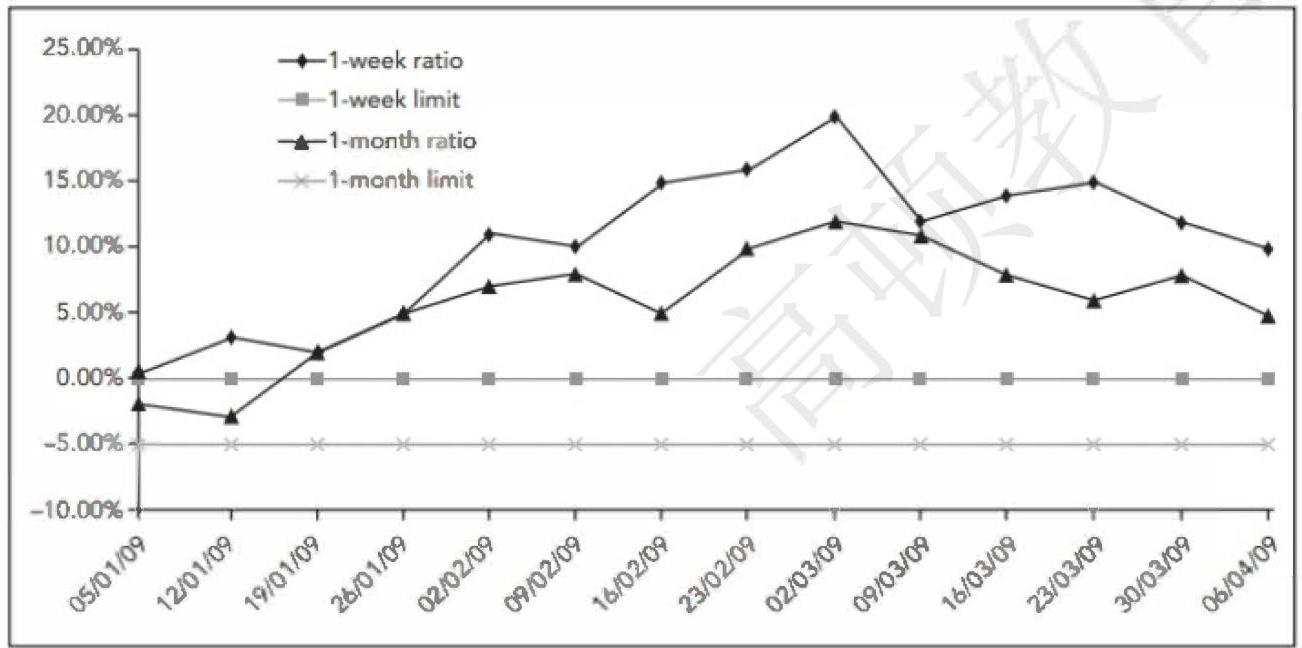
\includegraphics[width=0.9\textwidth]{images/report2.jpg}
        \end{center}
    
    \item Summary report example-part 3
    
    \begin{table}[htbp]
        \centering
        \begin{tabular}{lccc}
            \toprule
             & Current month & Previous month & Change \\
            \midrule
            LIQUIDITY RISK FACTOR & 22.2 & 25.1 & \(\downarrow\) \\ 
            LOAN-TO-DEPOSIT RATIO & 96\% & 93\% & \(\uparrow\) \\ 
            NET INTER-GROUP LENDING & (1,228) & (1,552) & \(\downarrow\)  \\ 
            \bottomrule
        \end{tabular}
    \end{table}
    \item Qualitative report: should be completed for Head Office Group Treasury on a monthly basis, for banking groups that operate across country jurisdictions and multiple subsidiaries.
        \begin{itemize}
        \item Assist the group to better understand the liquidity position in each country.
        \end{itemize}
    \end{itemize}
\item Qualitative report-Example



\begin{center}
    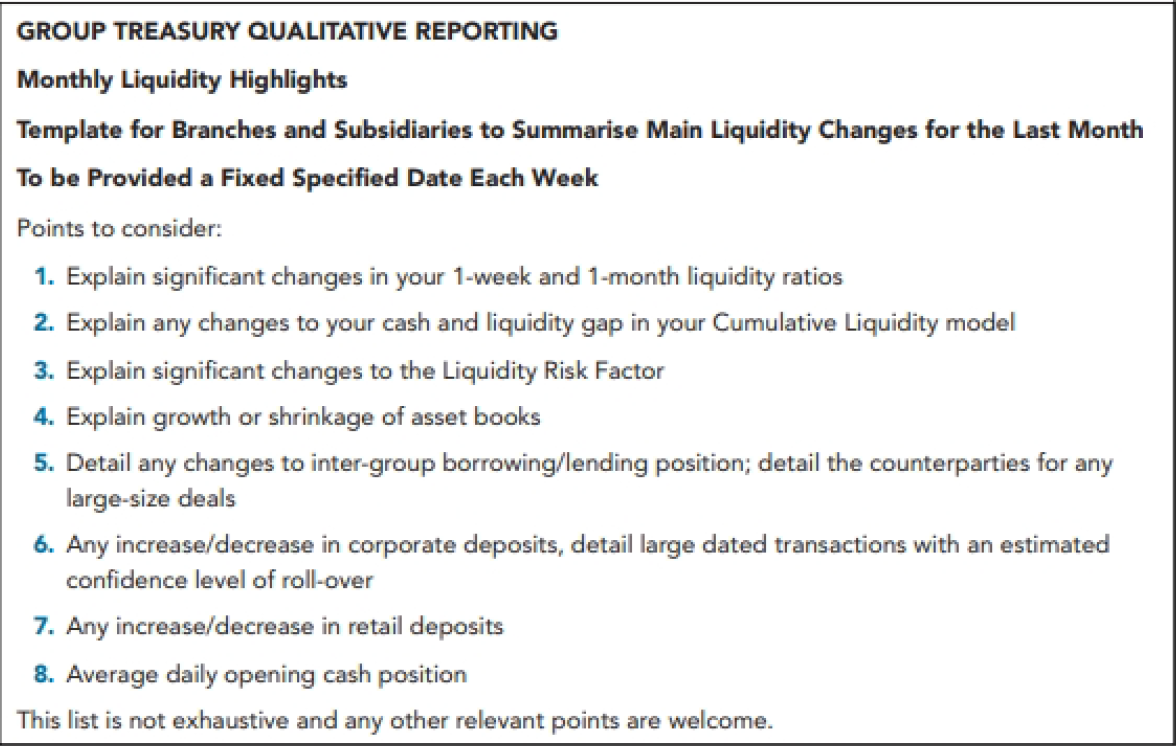
\includegraphics[width=0.9\textwidth]{images/reports1.png}
    \end{center}
\end{itemize}



\subsubsection{Benchmark liquidity reports for regulated banks in the UK}
\begin{itemize}
\item Deposit tracker report
\item Daily liquidity report
\item Funding maturity gap (mismatch) report
\item Funding concentration report
\item Undrawn commitment report
\item Liability profile
\item Wholesale pricing and volume
\end{itemize}



\subsubsection{Deposit tracker report}
\begin{itemize}
\item Definition: A simple report of the current size of deposits by customer type and forecast of what the level of deposits are expected to be going forward. LTD ratio is also provided.
\item Identified liquidity position: Loan to deposit ratio (LTD)
    \begin{itemize}
    \item Too high: may not have enough liquidity to cover any unforeseen fund requirements.
    \item Too low: may not be earning as much as it could be.
    \end{itemize}
\item Frequency: weekly and monthly
\end{itemize}

\begin{center}
    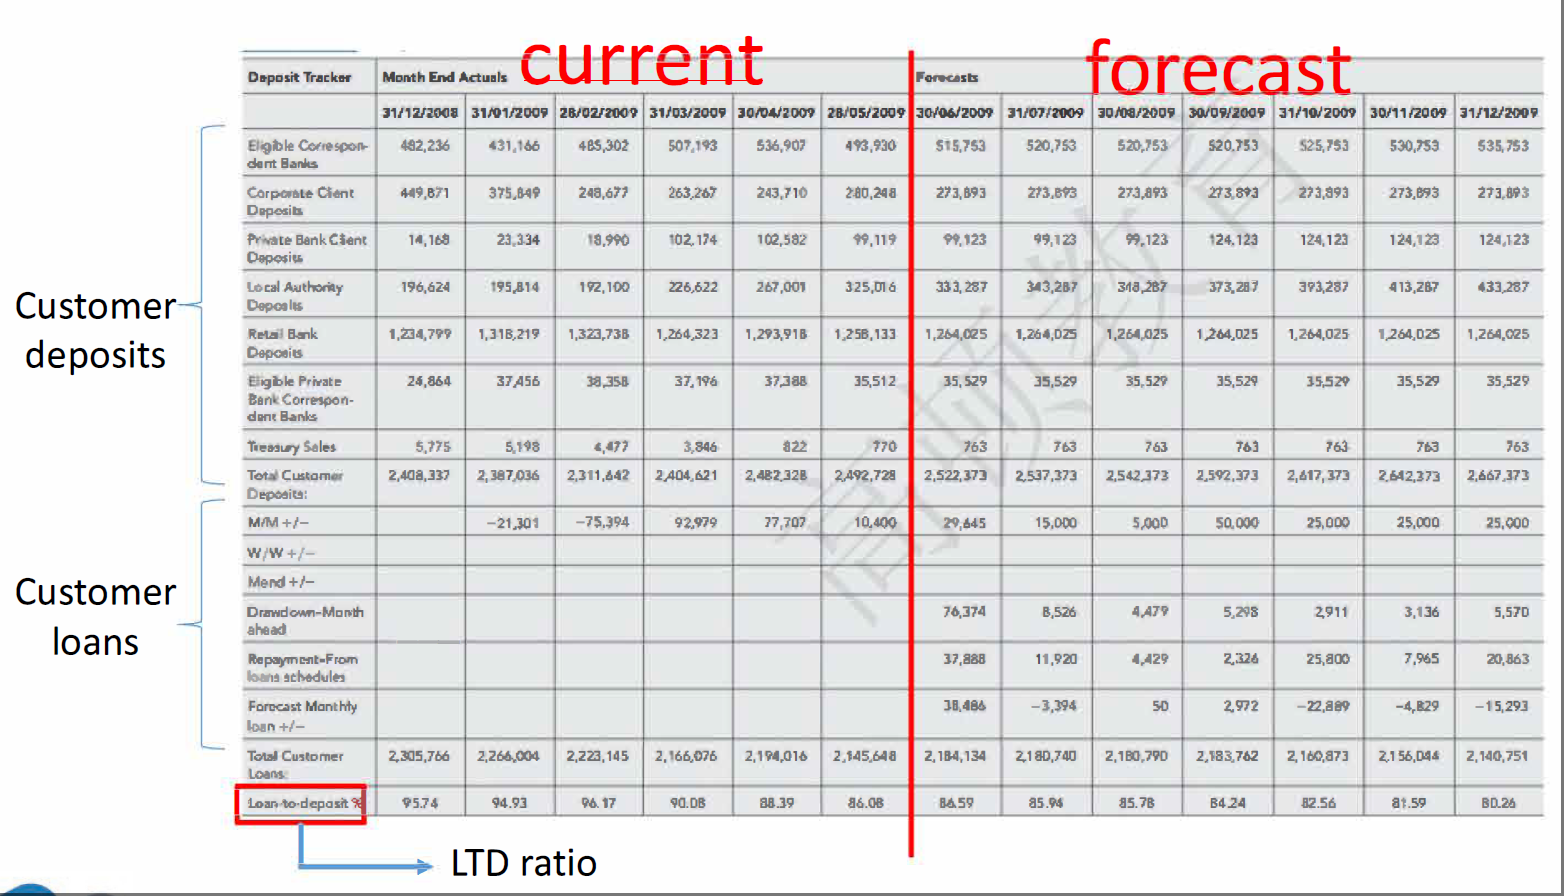
\includegraphics[width=0.9\textwidth]{images/LTD.png}
    \end{center}

\begin{center}
    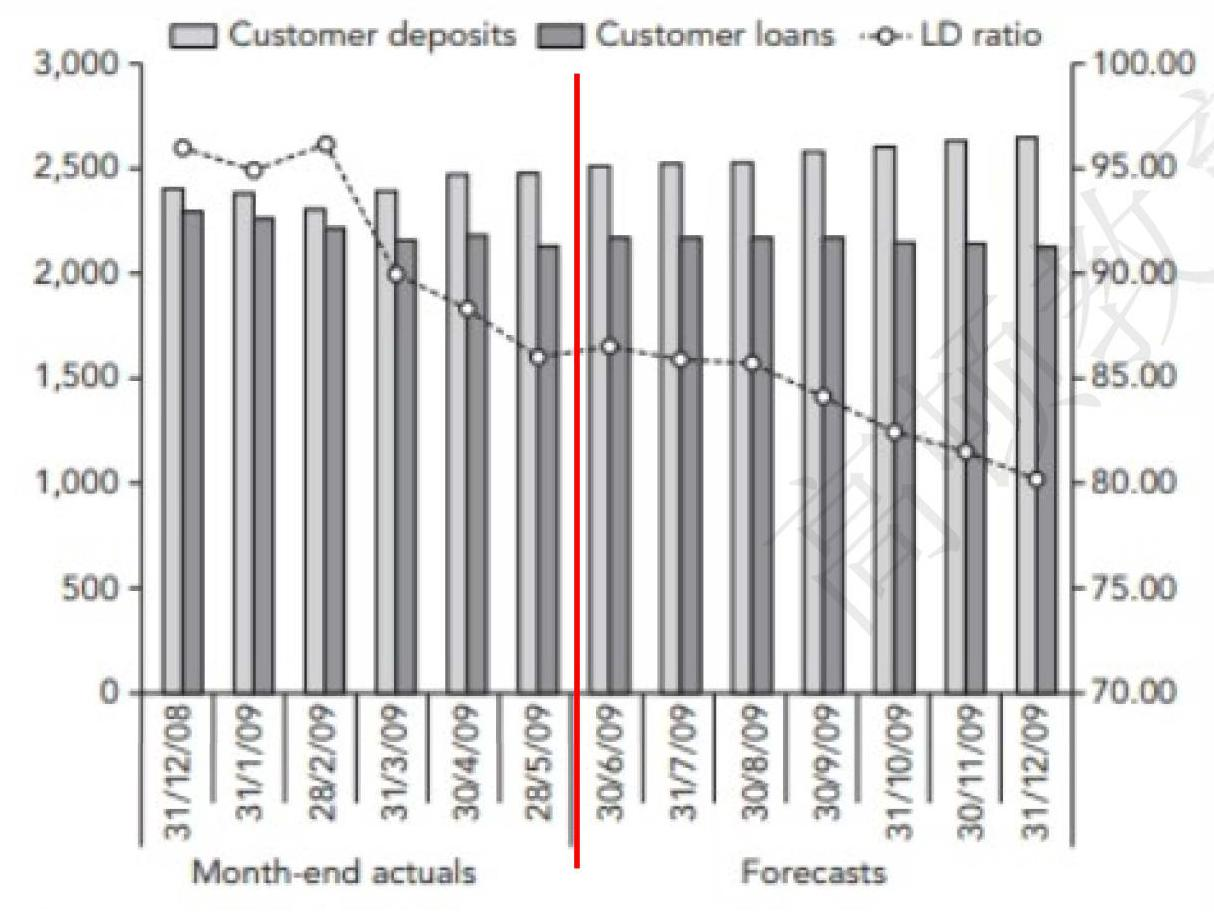
\includegraphics[width=0.9\textwidth]{images/DTR.jpg}
    \end{center}


\subsubsection{Daily liquidity report}
\begin{itemize}
\item Definition: A straightforward spreadsheet detailing the bank's liquid and marketable assets and liabilities, up to 1-year maturity. Each branch and subsidiary will complete this report.
    \begin{itemize}
    \item Input data: Summarizes the bank's liquid assets, liabilities by maturity/tenor.
    
  
    \item Output metrics: Provides an end-of-day of the bank's liquidity position like liquidity gap, cumulative cash gap.
    \end{itemize}
    
\item Frequency: daily
\item Input data


\begin{scriptsize}
    \begin{tabular}{@{}lrrrrrrrrrrrrr@{}}
    \toprule
    \textbf{ASSETS} & 1 Day & 2 Days & 1 Week & 2 Weeks & 1 Month & 2 Months & 3 Months & 6 Months & <1 Year & >1 Year & \textbf{Total} \\ \midrule
    Non-marketable Securities \& CDs & 0 & 0 & 0 & 0 & 0 & 0 & 0 & 0 & 0 & 0 & 0 \\
    Retail call a/c & 6,754 & 0 & 0 & 0 & 0 & 0 & 0 & 0 & 0 & 0 & 6,754 \\
    Retail time deposit & 432 & 3,533 & 0 & 4 & 4 & 4 & 4,529 & 9 & 1,619 & 420 & 23,749 & 34,299 \\
    Inter-Group call & 4,725 & 0 & 0 & 0 & 0 & 0 & 0 & 0 & 0 & 0 & 4,725 \\
    Inter-Group time & 19,199 & 89,848 & 281,434 & 90,150 & 135,378 & 73,895 & 60,768 & 21,379 & 5,912 & 244 & 778,207 \\
    Other bank call & 56,568 & 0 & 0 & 0 & 0 & 0 & 0 & 0 & 0 & 0 & 56,568 \\
    Other bank time & 5,465 & 148,347 & 188,620 & 7,833 & 89,500 & 30,020 & 0 & 25,319 & 128 & 83,985 & 579,217 \\
    Corporate call & 30,658 & 0 & 0 & 0 & 0 & 0 & 0 & 0 & 0 & 0 & 30,658 \\
    Corporate time & 13,936 & 112,975 & 35,335 & 53,432 & 10,923 & 159,894 & 133,718 & 63,182 & 116,551 & 1,365,637 & 2,065,583 \\
    Government bonds & 161,011 & 0 & 19,361 & 35 & 335 & 303 & 9 & 868 & 678 & 84,857 & 267,457 \\ \midrule
    \textbf{Total Assets} & 298,748 & 354,703 & 524,750 & 151,454 & 236,140 & 268,641 & 194,504 & 112,367 & 123,689 & 1,558,472 & 3,823,468 \\ \midrule
    \textit{Average remaining duration of assets} & & & \multicolumn{9}{l}{\textit{44.59 Months}} \\ 
    \bottomrule
    \end{tabular}
    \end{scriptsize}


    \begin{tabular}{lrrrrrrrrrrr}

        \toprule
        \textbf{Liabilities} & \textbf{1 Day} & \textbf{2 Days} & \textbf{1 Week} & \textbf{2 Weeks} & \textbf{1 Month} & \textbf{2 Months} & \textbf{3 Months} & \textbf{6 Months} & \textbf{< 1 Year} & \textbf{> 1 Year} & \textbf{Total} \\
   

        
        Retail call          & 97{,}482   & 0       & 0        & 0       & 0       & 0        & 0        & 0        & 0        & 0        & 97{,}482 \\
        Retail time          & 19{,}780   & 18{,}250 & 120{,}492 & 65{,}241 & 123{,}345 & 113{,}741 & 157{,}361 & 126{,}162 & 50{,}841  & 1{,}993   & 797{,}206 \\
        Inter-Group call     & 50{,}996   & 0       & 0        & 0       & 0       & 0        & 0        & 0        & 0        & 0        & 50{,}996 \\
        Inter-Group time     & 72{,}276   & 136{,}744 & 351{,}130 & 233{,}319 & 60{,}987  & 161{,}120 & 43{,}881  & 101{,}896 & 24{,}294  & 0        & 1{,}185{,}647 \\
        Other bank call      & 235{,}097  & 0       & 0        & 0       & 0       & 0        & 0        & 0        & 0        & 0        & 235{,}097 \\
        Other bank time      & 16{,}088   & 116{,}319 & 135{,}796 & 21{,}210  & 121{,}181 & 85{,}287  & 192{,}512 & 64{,}901  & 0        & 0        & 753{,}294 \\
        Corporate call       & 60{,}085   & 0       & 0        & 0       & 0       & 0        & 0        & 0        & 0        & 0        & 60{,}085 \\
        Corporate time       & 17{,}937   & 94{,}226  & 173{,}805 & 152{,}144 & 94{,}976  & 111{,}413 & 47{,}748  & 18{,}394  & 11{,}475  & 0        & 722{,}118 \\
        Government           & 3{,}689    & 6{,}005   & 58{,}163  & 109{,}046 & 37{,}671  & 204{,}339 & 54{,}477  & 31{,}341  & 5{,}902   & 1{,}122   & 511{,}755 \\

        \textbf{Total Liabilities} & 573{,}430  & 371{,}544 & 839{,}386 & 580{,}960 & 438{,}160 & 675{,}900 & 495{,}979 & 342{,}694 & 92{,}512  & 3{,}115   & 4{,}413{,}680 \\
        \addlinespace
        Undrawn commitments  & \multicolumn{11}{r}{273{,}242} \\
        Average remaining duration of liabilities & \multicolumn{11}{r}{7.72 Months} \\
        \bottomrule
        \end{tabular}
\item Output metrics

% 第一个表格
\begin{table}[htbp]
    \centering
    \caption{Cumulative Liquidity Report}
    \begin{tabular}{l*{9}{cccccccccc}}
        \toprule
        \multicolumn{1}{l}{} & \multicolumn{1}{c}{1 Day} & \multicolumn{1}{c}{2 Day} & \multicolumn{1}{c}{1 Week} & \multicolumn{1}{c}{2 Week} & \multicolumn{1}{c}{1 Month} & \multicolumn{1}{c}{2 Months} & \multicolumn{1}{c}{3 Months} & \multicolumn{1}{c}{6 Months} & \multicolumn{1}{c}{1 Year} \\
        \midrule
        Cumulative net cash balance & -111734 & -104480 & -301843 & -642230 & -738261 & -1040588 & -1884251 & -2122457 & -2099158 \\
        Other forecast inflows & {} & {} & {} & {} & {} & {} & {} & {} & {} \\
        Other forecast outflows & {} & {} & {} & {} & {} & {} & {} & {} & {} \\
        Cumulative cash gap & -111734 & -104480 & -301843 & -642230 & -738261 & -1040588 & -1884251 & -2122457 & -2099158 \\
        Counterbalancing capacity & 8676 & 8676 & 797674 & 804186 & 828686 & 877686 & 979996 & 1092696 & 1092696 \\
        Liquidity gap & -103058 & -95804 & 495831 & 161957 & 90426 & -162902 & -904256 & -1029761 & -1006462 \\
        Limit & {} & {} & {} & {} & {} & {} & {} & {} & {} \\
        Variance & -103058 & -95804 & 495831 & 161957 & 90426 & -162902 & -904256 & -1029761 & -1006462 \\
        \bottomrule
    \end{tabular}
\end{table}

% 第二个表格
\begin{table}[htbp]
    \centering
    \caption{Liquidity Metrics}
    \begin{tabular}{lcc}
        \toprule
         &  & Limit \\
        \midrule
        1-week Ratio & 11.13\% & 0.00\% OK \\
        1-month Ratio & 2.03\% & --5\% OK \\
        Liquidity Risk Factor & 3.85 &  \\
        \bottomrule
    \end{tabular}
\end{table}

\end{itemize}



\subsubsection{Funding maturity gap (mismatch) report}
\begin{itemize}
\item Definition: shows the maturity gap (maturity mismatch) per time bucket, for all assets and liabilities, with an adjustment for liquid securities.
    \begin{itemize}
    \item Identified liquidity position: cumulative liquidity cash flow of daily liquidity report is included in this report.
    \item 0-days survival horizon: required by Basel III.
    \end{itemize}
\item Frequency: monthly

\begin{center}
    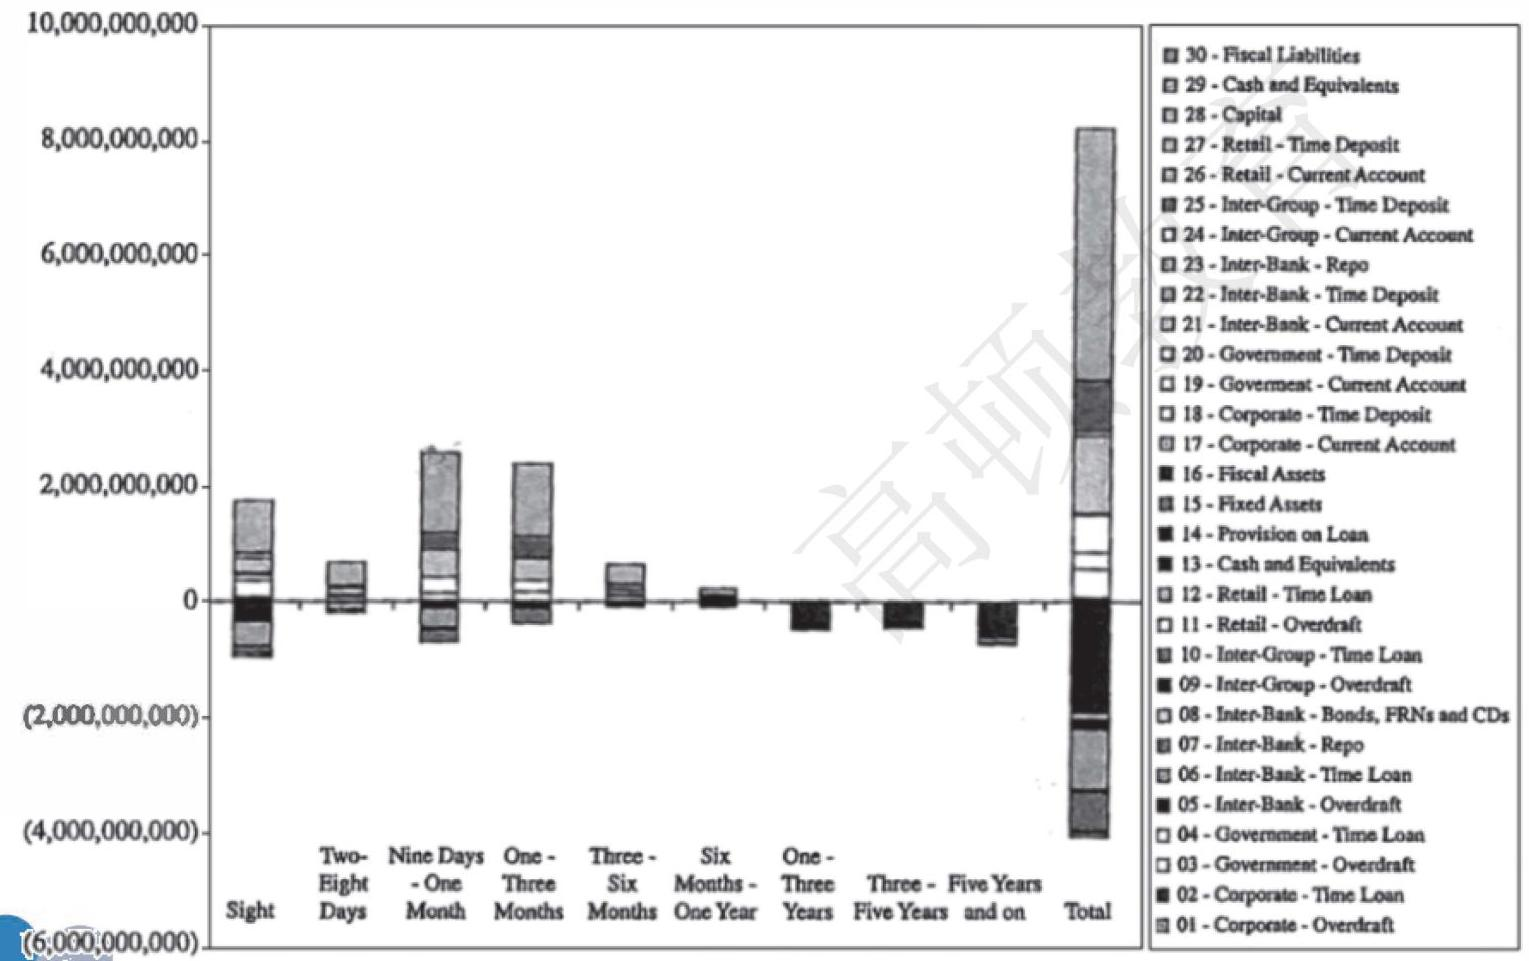
\includegraphics[width=0.9\textwidth]{images/mismatch.jpg}
    \end{center}

    \begin{center}
        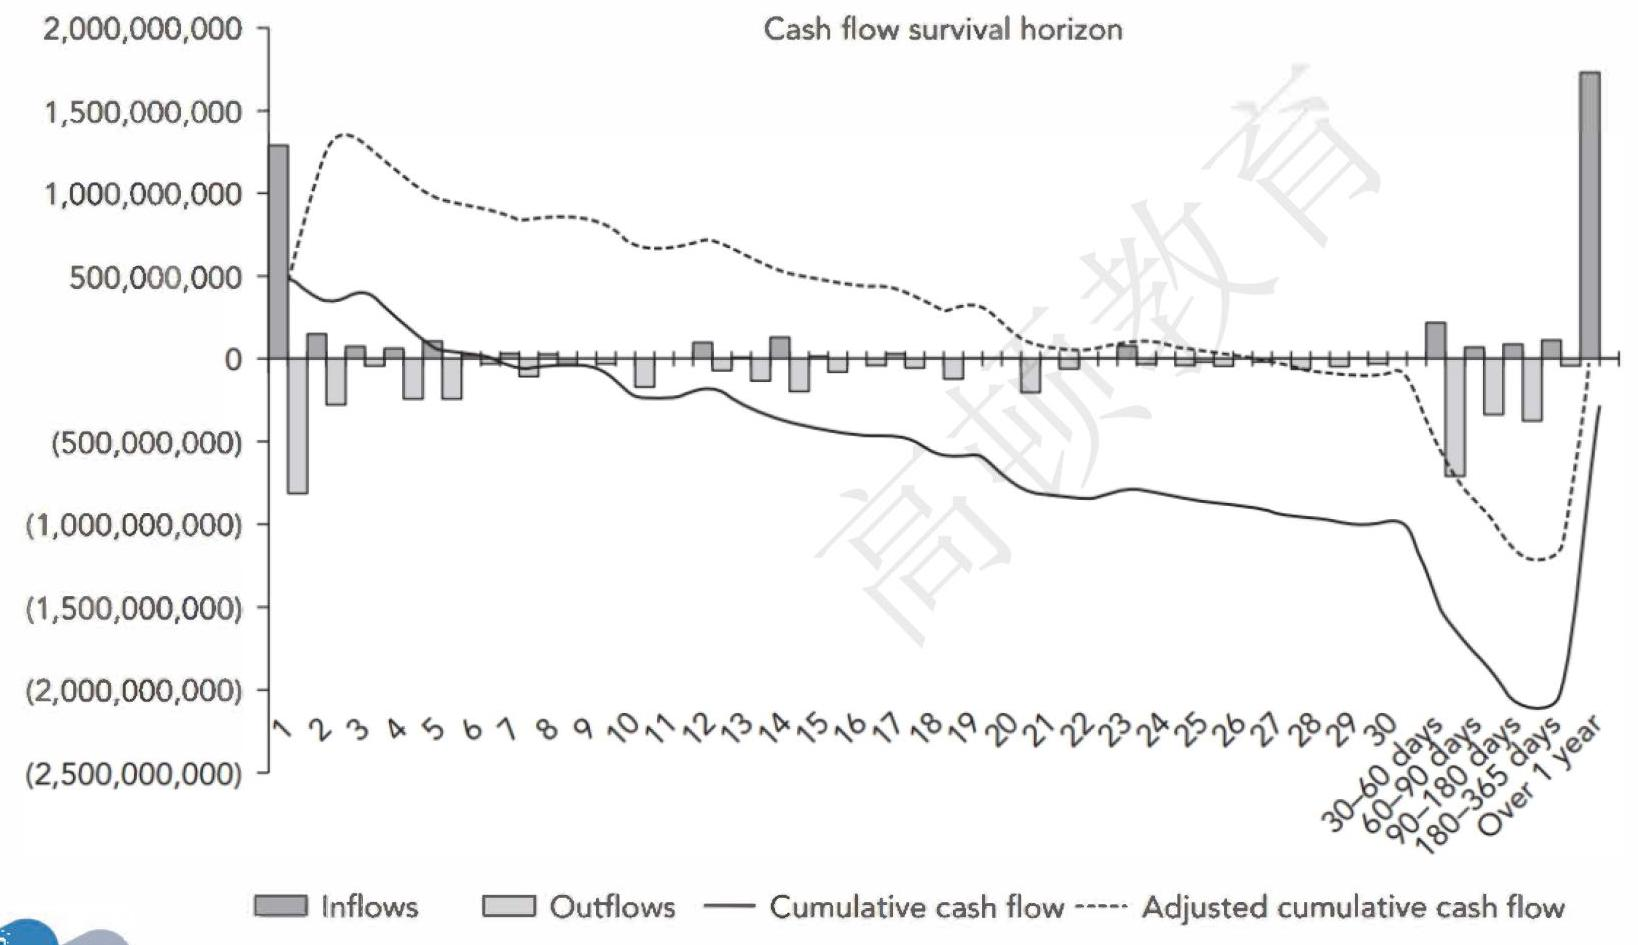
\includegraphics[width=0.9\textwidth]{images/mismatchreport.jpg}
        \end{center}
    
\end{itemize}



\subsubsection{Funding Concentration Report}
\begin{itemize}
\item Definition: Funding source concentration reports
\begin{itemize}
\item Funding diversity: A bank should not become over-reliant on a single source, or sector, of funds. A deposit of 5\% of total liabilities should be treated as large by ALCO.
    \begin{itemize}
    \item The way to increase diversity: Increase its liabilities rather than asking the depositor to remove some of the fund to avoid damaging the relationship.
    \end{itemize}
    
\item Frequency: monthly

%这里有个表格
\end{itemize}
\end{itemize}



\subsubsection{Undrawn Commitment Report}
\begin{itemize}
\item Definition: shows the existence of undrawn commitment trend over time.
    \begin{itemize}
    \item Off balance sheet products: potential stress points for a bank's funding requirement and exacerbate funding shortages at the wrong time.
        \begin{itemize}
        \item Liquidity lines, revolving credit facilities, letters of credit, guarantees
        \end{itemize}
    \end{itemize}
\item Frequency: monthly

\begin{center}
    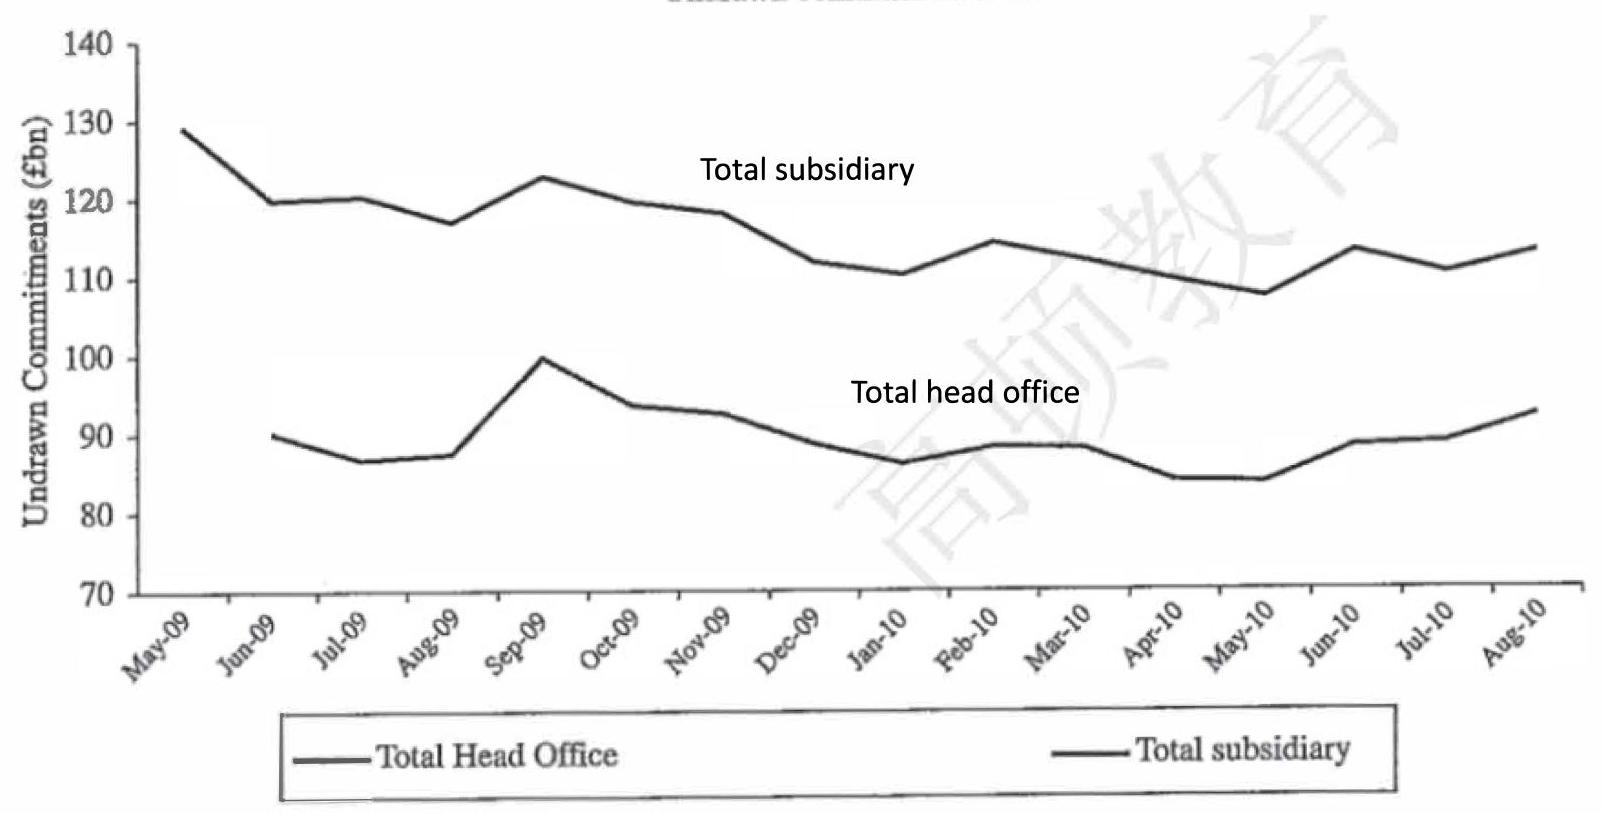
\includegraphics[width=0.9\textwidth]{images/Undrawn.jpg}
    \end{center}

\end{itemize}



\subsubsection{Liability Profile}
\begin{itemize}
\item Definition: A simple breakdown of the share of each type of liability at the bank. The report format can be set to the user's desired choice.
    \begin{itemize}
    \item The total liabilities are made of the following categories:
        \begin{itemize}
        \item Customers: individual and large enterprises
        \item Repo
        \item Asset-backed securities
        \item Unsecured wholesale, etc.
        \end{itemize}
        
    \end{itemize}   
\item Frequency: monthly
\begin{center}
    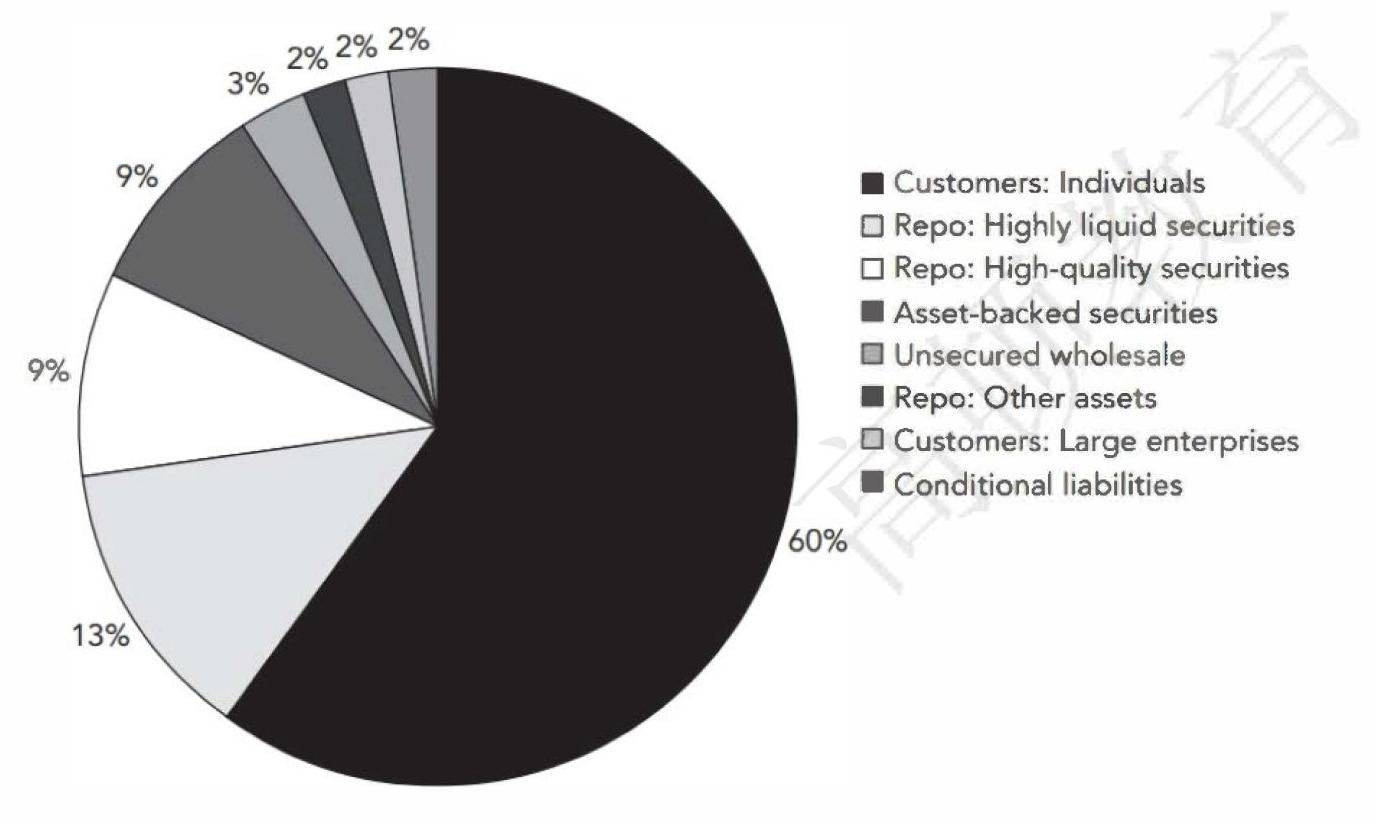
\includegraphics[width=0.9\textwidth]{images/LiabilityProfile.jpg}
    \end{center}



\end{itemize}



\subsubsection{Wholesale Pricing and Volume}
\begin{itemize}
\item Definition: a report of firm-specific yield curve.
    \begin{itemize}
    \item Liquidity strength can be gleaned from looking at a bank's funding costs, and the composition of its funding by product.
    \item An early warning of a particular bank experiencing funding stress if its funding yield curve is rising materially above that of its peer group.
    \end{itemize}
\item Frequency: at least quarterly

\begin{center}
    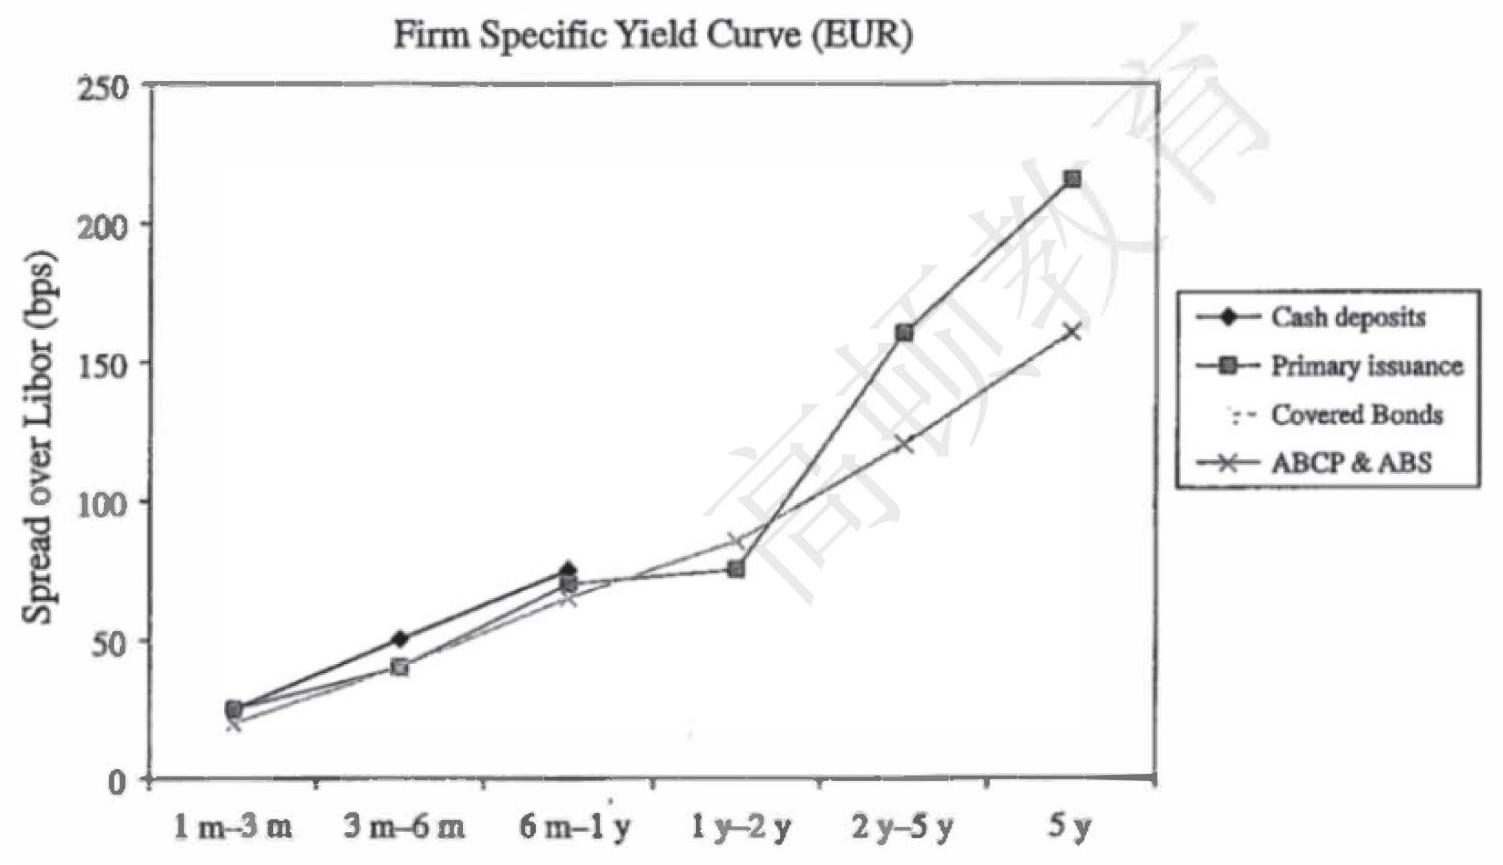
\includegraphics[width=0.9\textwidth]{images/Wholesale.jpg}
    \end{center}

\end{itemize}


\subsection{Contingency Funding Planning Ch11}


\subsubsection{Introduction}
\begin{itemize}
\item Definition: Contingency Funding Plan (CFP) provides a structured approach for developing and implementing the institution's financial and operational strategies for effectively managing such contingent liquidity events during periods of severe market and financial stress.
    \begin{itemize}
    \item Business as usual funding (BAU) : low-impact, highprobability event.
    \item Contingency Funding Plan （CFP）: high-impact, lowprobability events.
    \end{itemize}
\end{itemize}


\subsubsection{Relationship with liquidity stress test}
\begin{itemize}
\item Link the stress test results and other related information as  inputs to the CFP governance.
\item Liquidity stress testing is helpful to establish limits and escalation levels.
\end{itemize}


\subsubsection{Key design considerations}
\begin{itemize}
\item Aligned to business and risk profiles
    \begin{itemize}
    \item Aligning the institutions' risk appetite to the CFP framework, through quantifiable EWls, limits, and escalation levels.
    \item Refresh CFP as the institution's business and risk profile changes over time. Leading institutions develop the CFP to be more forward looking and flexible.
        \begin{itemize}
        \item Corporate and business strategies change
        \item New products and services
        \item Macroeconomic and market environments
        \end{itemize}
    \end{itemize}
\item Integrated with broader risk management frameworks
    \begin{itemize}
    \item An integrated part of the institution's liquidity risk management and firm-wide risk management frameworks:
        \begin{itemize}
        \item Enterprise risk management (ERM)
        \item Capital management
        \item Business continuity
        \item Crisis management
        \end{itemize}
    \end{itemize}
\item Operational and actionable, but flexible playbook
    \begin{itemize}
    \item A menu of possible contingency actions that management can undertake in different stress scenarios and at graduated levels of severity.
    \item As a playbook, the effectiveness of the CFP lies in its operational readiness.
    \end{itemize}
\item Inclusive of appropriate stakeholder groups
    \begin{itemize}
    \item Involvement of appropriate stakeholder groups:
        \begin{itemize}
        \item Asset liability committee (ALCO)
        \item Risk and capital committee
        \item Investment committee
        \item Business units:
            \begin{itemize}
            \item Finance, corporate treasury, risk, operations , technology
            \end{itemize}
        \end{itemize}
    \item Ensure internal and external stakeholders to remain confident in the institution's financial strength.
    \end{itemize}
\item Supported by a communication plan
    \begin{itemize}
    \item In any crisis, the coordinated and timely communication of information to stakeholders is critical.
    \item External communication to clients, analysts, counterparties, and regulators with timely and accurate information is critical.
        \begin{itemize}
        \item Help to reinforce confidence in the institution and mitigate potential risk that rumors, and fears do not further precipitate and adversely impact the institution.
        \end{itemize}
    \end{itemize}
\end{itemize}


\subsubsection{Key components of a CFP framework}
\begin{itemize}
\item Governance and oversight

\begin{table}[htbp]
    \centering
    \begin{tabular}{cc}
        \toprule
        \multicolumn{1}{>{\color{blue}}l}{Roles} & \multicolumn{1}{>{\color{blue}}l}{Responsibilities} \\
        \midrule
        Corporate treasury & \makecell{\checkmark In consultation with the CFO and others, may invoke CFP and convene Liquidity Crisis Team.} \\
        \midrule
        Liquidity crisis team(LCT) & \makecell{\checkmark Designing the CFP \\ \checkmark Providing recommendations on CFP actions \\ \checkmark Central point of contact, ensure effective coordination across the organization as well as with external stakeholders} \\
        \midrule
        Management committee & \makecell{\checkmark Oversight of LCT \\ \checkmark Reviewing specific recommendations for and coordination of CFP actions} \\
        \midrule
        Board of directors & \makecell{\checkmark An advisor and counsel to LCT and management \\ \checkmark Evaluating CFP actions} \\
        \bottomrule
    \end{tabular}
\end{table}
\item Scenarios and liquidity gap analysis
    \begin{itemize}
    \item Align the CFP stress scenarios to liquidity stress testing framework, as well as to other frameworks such as the recovery and resolution plans.
    \item CFP may contain additional liquidity-related stress scenanos.
        \begin{itemize}
        \item lntraday debit cap with Fedwire is exceeded
        \item Specific counterparties fail
        \item Federal Home Loan Bank funding becomes unavailable
        \end{itemize}
    \end{itemize}
    
\item Contingent actions: help strengthen the institution's liquidity
position.
    \begin{itemize}
    \item Reducing the amount of lending activity
    \item  Offering higher rates on deposits
    \item Choosing not to reinvest securities when they mature
    \item Increasing securitization activities
    \item Disposing of liquid assets
    \item Issuing subordinated debt
    \item Disposing of business unit
    \end{itemize}
\item Monitoring and escalation
    \begin{itemize}
    \item Early warning indicators
    \item Market and business factors
        \begin{itemize}
        \item Spike in market volatility (e.g., VIX)
        \end{itemize}
        
    \item Liquidity health measures
        \begin{itemize}
        \item Projected net funding requirements current unused funding capacity
        \item Non-core funding to long-term assets
        \item Overnight borrowings to total assets
        \item Short-term liabilities to total assets
        \item Funding sources concentration
        \item Funding maturity profile
        \item Used capacity to total borrowing capacity
        \item Liquid assets to volatile liabilities
        \item Unpledged eligible collateral to total assets
        \item Loans to commitments
        \end{itemize}
    \item Escalation Levels: 3 to 5 escalation levels
        \begin{itemize}
        \item Level 1: Triggered by stress test results indicating a greater decline in liquidity than the institution's risk appetite targets and/or a shift in the market's perception of the institution.
        \item Level 2: Triggered when institution experiences noticeable markets and/or idiosyncratic events that are adversely impacting its business and liquidity risk profile.
            \begin{itemize}
            \item Focus on immediate and short-term horizon.
            \end{itemize}
        \item Level 3: Triggered when dramatic steps should be taken to stabilize the liquidity position.
            \begin{itemize}
            \item Focus on survival.
            \end{itemize}
        \end{itemize}
    \end{itemize}
\item Data and reporting
    \begin{itemize}
    \item Reports capture intraday liquidity positions, track exposure to contingent liabilities, and monitor capacity usage in funding sources.
    \item Reports convey methods used to determine liquidity coverage for upcoming liabilities and funding.
    \item Increasing the frequency of liquidity management reporting benefit the institution.
    \end{itemize}
\end{itemize}





 